\section{The Exocentric vision issue}
\label{sec:exo}
\subsection{Why exocentric vision?}
Teleoperated mobile robots prove to be extremely useful 
when there is the need for performing operations in places that 
are inaccessible or dangerous for human beings - e.g. 
search-and-rescue missions within unknown regions or into 
collapsed buildings, caves, etc.
%
The supervisors' research group has been widely involved 
during the last years in such a field: \cite{livatino2010}.
%
As testing platform, they have been using \textit{3morduc},
a differential-driven mobile robot - showed in figure \ref{fig:3morduc} -
equipped with a pair of \textit{Videre Design} \cite{videredesign} 
stereo cameras and a laser scanner. They have been focused 
mainly on the making of a reliable hardware and software 
infrastructure which could make a remote operator able to drive 
the 3morduc in comfort.
%% parlare dei campi di ricerca coinvolti?
%
\begin{figure}[!h]
  \begin{center}
    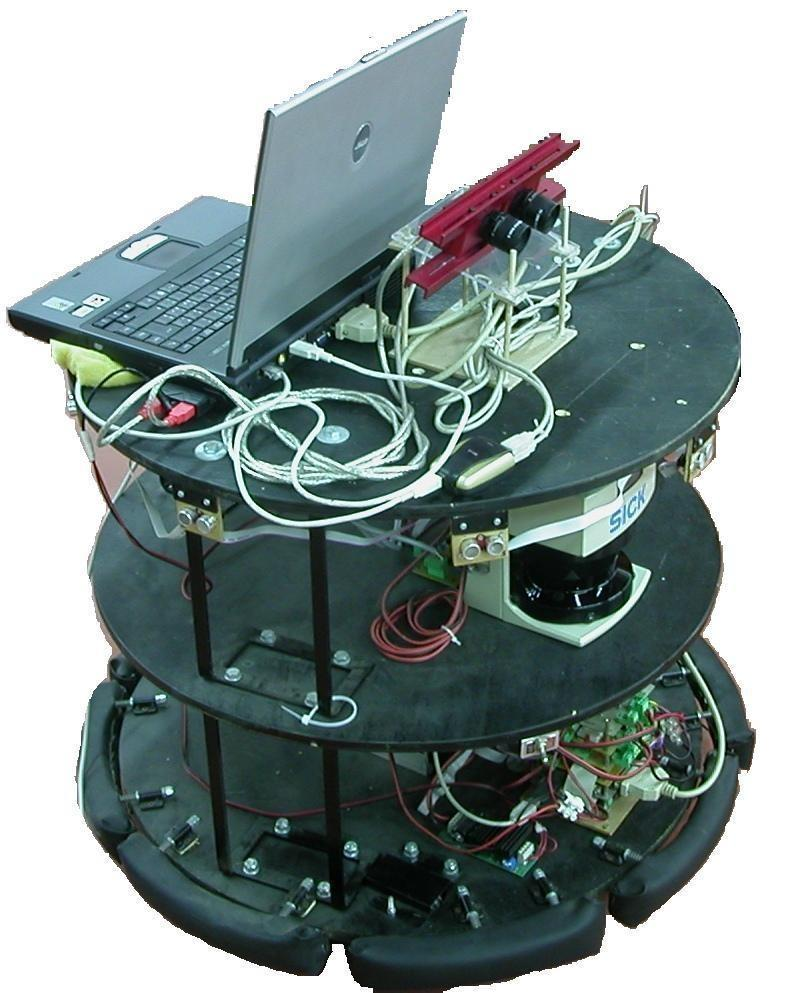
\includegraphics[width=200pt]{img/3morduc.jpg}  %robot pic
    \caption{The 3morduc robotic platform}
    \label{fig:3morduc}
  \end{center}
\end{figure}
%
Indeed, our work will focus on \textit{robot-operator interaction} and, 
hence, on how to improve such interaction. 
%
Analyzing previous work and data produced by the supervisors' 
research group, it emerges that the stereo cameras mounted on 
top of 3morduc, were used to provide the remote operators a 
\textit{first-person} point of view. In literature, such a 
system is also called an \textit{egocentric} vision system.
%

%
According to \cite{sugimoto}, \textit{by observing the camera image 
without an efficient human interface system, the operator 
tends to misinterpret the robot's position and direction}. This is 
due to the fact that  \textit{it's difficult for an
operator not accustomed to the vehicle to estimate the
vehicle's position and direction and the distances to a
target strictly based on camera images from the first person 
viewpoint}.
%
In order to improve the interaction between the robot and the operator 
an exocentric camera would be effective since it would provide a 
representation of the robot in the operating environment and, thus, 
a better understanding of where the robot is located into the environment 
and its actual direction.
%
Unfortunately the use of an exocentric camera is not straightforward: 
for example, it could be mounted on a rear-mounted protuberance of the 
robot, but such a protuberance would terribly limit the robot activity and 
its moving abilities.
%
To avoid such complications, \cite{sugimoto} proposes 
\textit{Time Follower's}, an approach to provide a \textit{virtual exocentric 
view} of a mobile robot.
%
\subsection{Time Follower's: an overview}
Time Follower's aims at providing an exocentric view of a mobile 
robot using an egocentric-mounted camera. The approach is simple: it is 
based on the use of previously recorded first-person images to provide 
comprehensible third-person imagery. A 3D representation of the robot 
is overlapped to such images in order to get the work done. A graphical
representation of the system is depicted in figure \ref{fig:exocentric}, 
while figure \ref{fig:virtualexocentric} shows an example of what appears 
to the end user.
%
\begin{figure}[!h]
  \begin{center}
    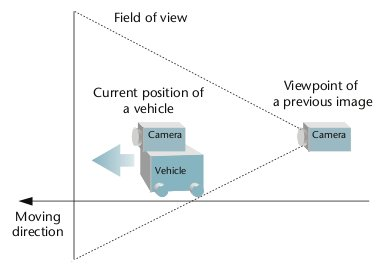
\includegraphics[width=200pt]{img/exocentric_vision.jpg}
    \caption{The 3morduc robotic platform}
    \label{fig:exocentric}
  \end{center}
\end{figure}
%
\begin{figure}[!h]
  \begin{center}
    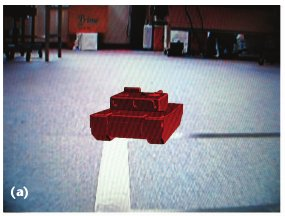
\includegraphics[width=200pt]{img/virtual_exocentric.jpg}  %robot pic
    \caption{A virtual exocentric vision example}
    \label{fig:virtualexocentric}
  \end{center}
\end{figure}
%

%
Key issues of such a system are:
\begin{itemize}
\item how to choose the \textit{best} image
\item how to determine the \textit{right} place to draw the robot
\end{itemize}
%
As for the first issue, the \textit{best} image is the one that allows 
the generation of the \textit{most comprehensible} external robot view.
\cite{sugimoto} provides a set of three effective metrics to 
determine which, of a set of previously recorded images, is the 
one to be chosen.
%
Once the image is chosen, where to overlap the 3D robot representation 
is quite complex. It is not only a matter of \textit{where} draw the robot
on the image, but also of \textit{how} to set up lighting, robot dimensions,
perspective to make the end user not aware of the fact that what he is
seeing is not the actual environment.
%
We will analyze such aspects in the following of this report.

%% Non solo, una immagine precedente, contiene informazioni ambientali piu' 
%% ampie rispetto a quelle di una camera montata sul posteriore del robot.
